%\section{Mengenai dokumen ini}
%Blah

\section{Pengenalan Quartus Prime}

Quartus Prime merupakan perangkat lunak CAD (computer-assisted design)
yang digunakan untuk desain rangkaian digital. Quartus Prime dikembangkan
oleh Altera. Versi Lite dari Quartus Prime dapat diunduh secara gratis
pada laman Altera\footnote{\url{http://dl.altera.com/?edition=lite}}.
Quartus Prime dapat dijalankan pada
platform Windows dan Linux.
Jendela utama dari Quartus Prime Lite dapat dilihat pada Gambar
\ref{fig:main_window}.

\begin{figure}
\centering
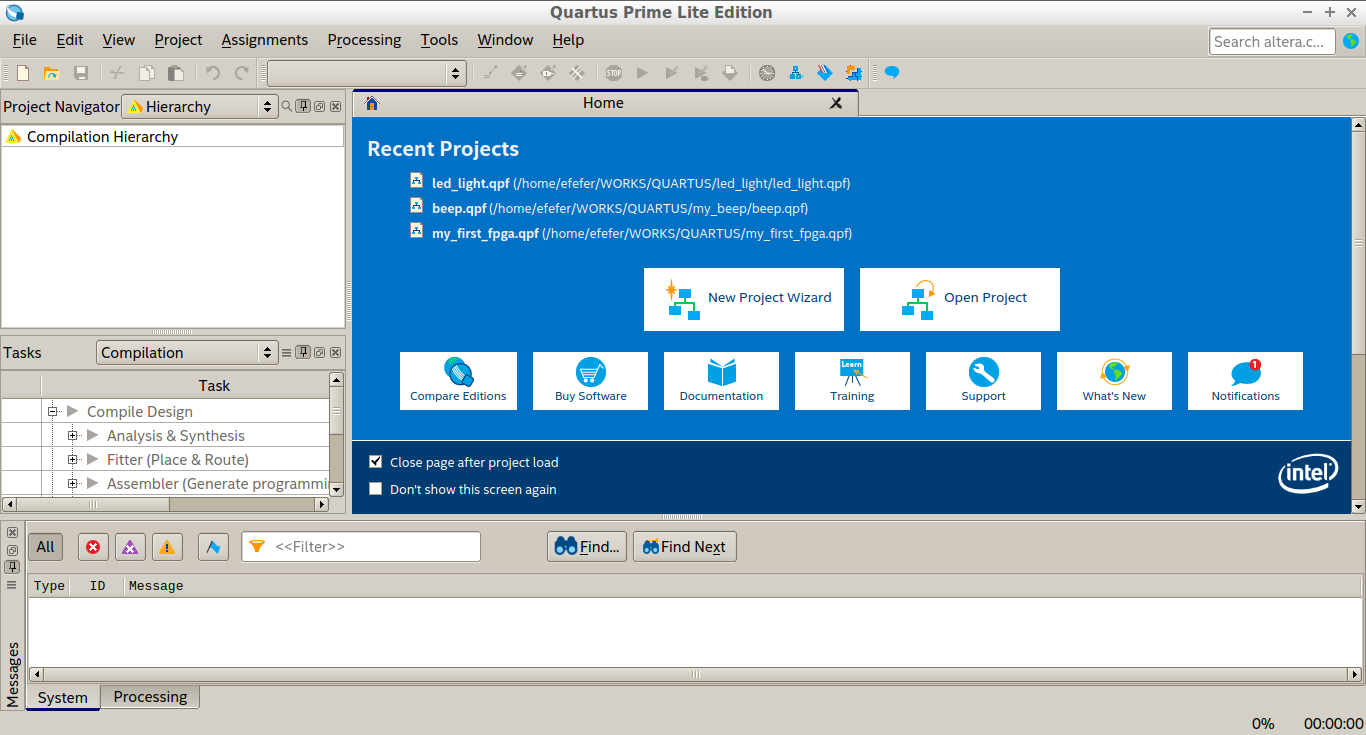
\includegraphics[width=\textwidth]{images/FirstOpen.png}
\par
\caption{Tampilan jendela utama Quartus Prime Lite}\label{fig:main_window}
\end{figure}

Dengan menggunakan CAD, setidaknya ada dua cara untuk
mendesain rangkaian digital:
\begin{itemize}
\item \textit{schematic capture}, dengan membuat skematik dari rangkaian yang
diinginkan.
\item menggunakan Hardware Description Language (HDL).
Dua jenis HDL yang paling populer adalah Verilog dan VHDL.
Kedua bahasa tersebut telah diadopsi sebagai IEEE Standard.
Pada tulisan ini akan digunakan Verilog.
\end{itemize}
